\subsection{One dimensional hydrogen chain}
%Let us consider the following single band model Hamiltonian,
We here apply the downfolding approach to a one dimensional \textit{ab initio} system,  a10-sites hydrogen chain with periodic boundary condition.  We consider the cases where the inter-atomic distance is relatively large, such that the system could be well described by a single Hubbard model (primarily $s$ orbitals). The inter-atomic distance is varied from 1.5 to 3.0 \AA. 
\begin{eqnarray}\label{eq:h4model}
H &=& \sum_{i}\left\{-t[c^{\dagger}_{i\sigma}c_{i+1\sigma} +h.c.]+ Un_{i\uparrow}n_{i\downarrow}\right\} + C\,.
\end{eqnarray}
%\begin{eqnarray}\label{eq:h4model}
%H &=& \sum_{i}\left\{-t[c^{\dagger}_{i\sigma}c_{i+1\sigma} +h.c.]+ Vn_{i}n_{i+1} + Un_{i\uparrow}n_{i\downarrow}+ J\vec \sigma_{i}\cdot \vec \sigma_{i+1}\right\} + C\,.
%\end{eqnarray}
%Here, $c_{i}$'s are Wannier orbitals generated from Kohn-Sham orbitals. We consider the case where the inter-atomic distance is relatively large, such that the system could be well described by a single band.  We start from the 4-site hydrogen chain with bond length equals to 2\AA with periodic boundary condition. We construct the Wannier orbitals by a unitary transformation of the four lowest energy Kohn-Sham states obtained from DFT/PBE calculation (2 occupied and 2 unoccupied). Fig.~\ref{fig:h4orb} shows the selected Kohn-Sham orbitals and constructed Wannier orbitals. 
%\begin{figure}[hbt]
%\centering
%\subfigure[KS 1]{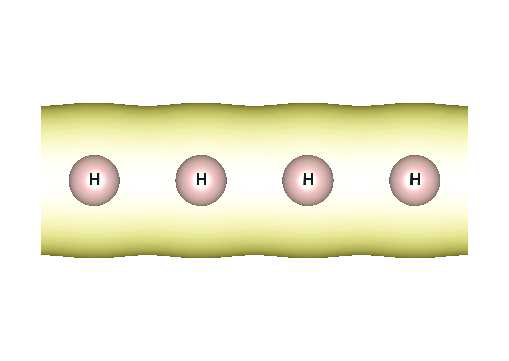
\includegraphics[width=0.20\linewidth]{./Figures/h4_ks1.png}}\quad
%\subfigure[KS 2]{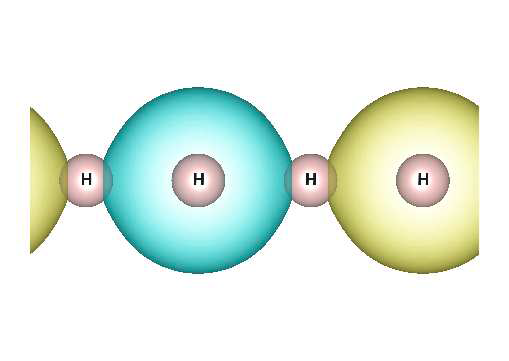
\includegraphics[width=0.20\linewidth]{./Figures/h4_ks2.png}}\quad
%\subfigure[KS 3]{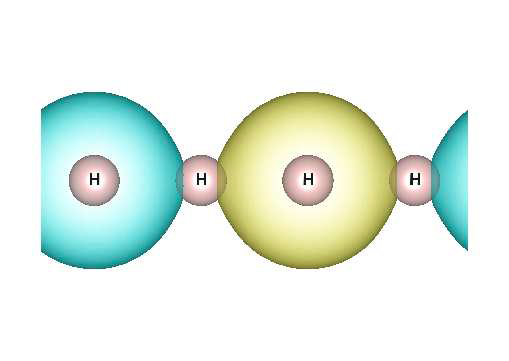
\includegraphics[width=0.20\linewidth]{./Figures/h4_ks3.png}}\quad
%\subfigure[KS 4]{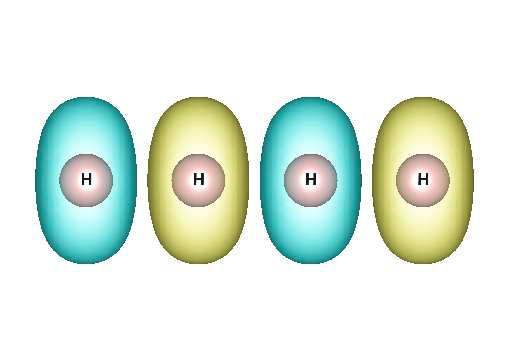
\includegraphics[width=0.20\linewidth]{./Figures/h4_ks4.png}}
%\\
%\subfigure[Wannier 1]{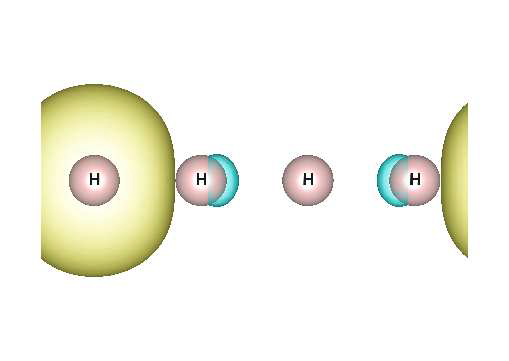
\includegraphics[width=0.20\linewidth]{./Figures/h4_wan1.png}}\quad
%\subfigure[Wannier 2]{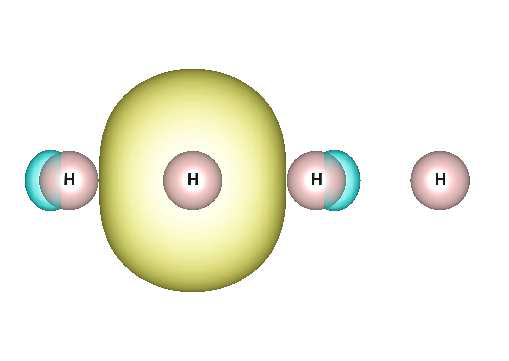
\includegraphics[width=0.20\linewidth]{./Figures/h4_wan2.png}}\quad
%\subfigure[Wannier 3]{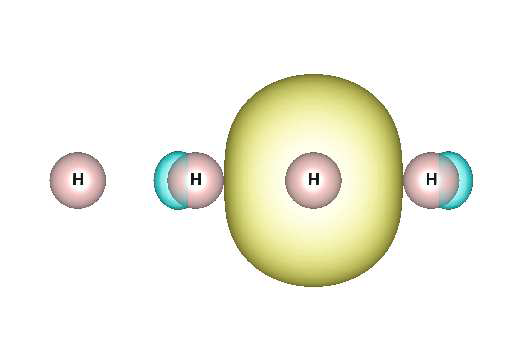
\includegraphics[width=0.20\linewidth]{./Figures/h4_wan3.png}}\quad
%\subfigure[Wannier 4]{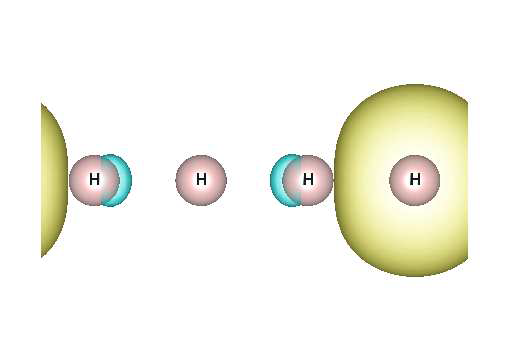
\includegraphics[width=0.20\linewidth]{./Figures/h4_wan4.png}}
%\caption{Kohn-Sham orbitals (upper panel) from DFT calculations with PBE exchange-exchange correlation functional, and Wannier orbitals (lower panel) constructed through a unitary transformation of Kohn-Sham orbitals.}\label{fig:h4orb}
%\end{figure}

%We will use the mentioned E-AIDMD method to downfold the ab initio system into the model Hamiltonian in Eq.~\eqref{eq:h4model} by matching the single-body energy spectra and the 1-body and 2-body reduced density matrices. The model Hamiltonian is solved by exact diagonization, whereas the \textit{ab initio} system is solved using diffusion Monte Carlo method with single Slater-Jastrow trial wave functions. 
%
%In our calculations, we used energies and RDMs of the following three states:
%\begin{subequations}
%\begin{eqnarray}
%S=0: \quad E = -2047.8(6) \text{mHa}; \\
%S=1: \quad E = -2038.9(5) \text{mHa}; \\
%S=2: \quad E = -1957.8(3) \text{mHa}.
%\end{eqnarray}
%\end{subequations}
%where S is the total angular moment of such the four-site hydrogen chain. In order to understand the relative importance of various two-body terms: (a) the on-site Hubbard interaction -- $\hat U$; (b) nearest neighbor Coulomb interaction -- $\hat V$; (c) nearest neighbor exchange -- $\hat J$, we compare the parameters obtained when downfolding the system to the following three different models with different two-body interactions,
%\begin{itemize}
%\item [(a)] \textbf{UVJ} model: onsite Hubbard interaction(U), nearest neighbor Coulomb (V) and exchange (J);
%\item [(b)] \textbf{UV} model: onsite Hubbard interaction(U), nearest neighbor Coulomb (V);  J is set to zero. 
%\item [(c)] \textbf{U} model: onsite Hubbard interaction(U). V and J are set to zero. 
%\end{itemize}
%
%The quality of downfolding is measured by the relative error of the two-body reduced density matrices, and the error of the eigen energies of the three states.
%\begin{eqnarray}
%R_{err} =\sqrt{\frac{\sum_{i,j,k,l}(M_{ijkl}^\text{ab initio} - M_{ijkl}^\text{model})^{2}}{\sum_{i,j,k,l}(M^\text{ab initio}_{ijkl})^{2} }}, \quad
%\Delta E = \sqrt{\sum_{i}|E_{i}^\text{ab initio} - E_{i}^{\text{model}}|^{2}}\,.
%\end{eqnarray}
%The resulting effective parameters are showed in Table.~\ref{tab:effm_hchain}. We see that all the three models can match the \textit{ab initio} data accurately. U model has relatively larger error in energy, but it is still comparable to the stochastic error from QMC (0.3 $\sim$ 0.5 mHa).
%
%\begin{table}[hbt]
%\centering
%\begin{tabular}{||l|c|c|c|c||c|c||}
%\hline
%Model & t & U & V & J & err(RDM) & err(energy)\\
%\hline
%\hline
%UVJ & 23.68 & 34.58 & 0.03 & -3.11 & 0.25\% & $10^{-13}$\\
%UV & 32.76 & 130.63 & 65.31 & / & 0.75\% & $10^{-13}$\\
%U & 37.45 & 114.62 & / & / & 0.26\% & $1.8$\\
%\hline
%\end{tabular}
%\caption{Parameters of effective Hamiltonian [mHa], and error of RDMs and energies [mHa].}\label{tab:effm_hchain}
%\end{table}
%
%%\subsection{Transferability of the model parameters to larger systems} 
%\begin{figure}[hbt]
%\centering
%\subfigure[]{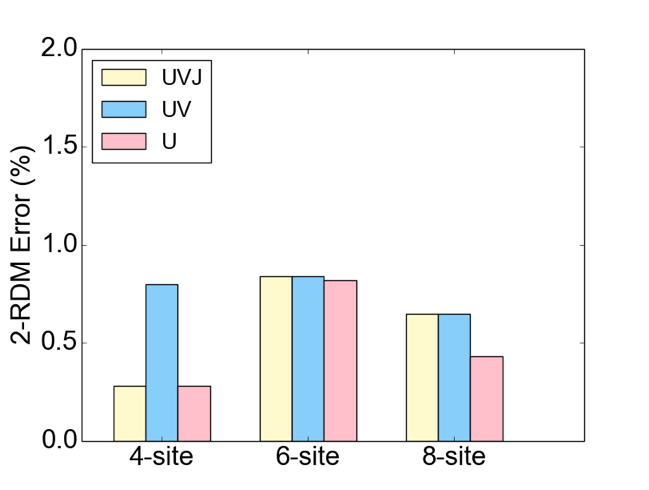
\includegraphics[width=0.40\linewidth]{h4_transfer_rdm.png}}
%\subfigure[]{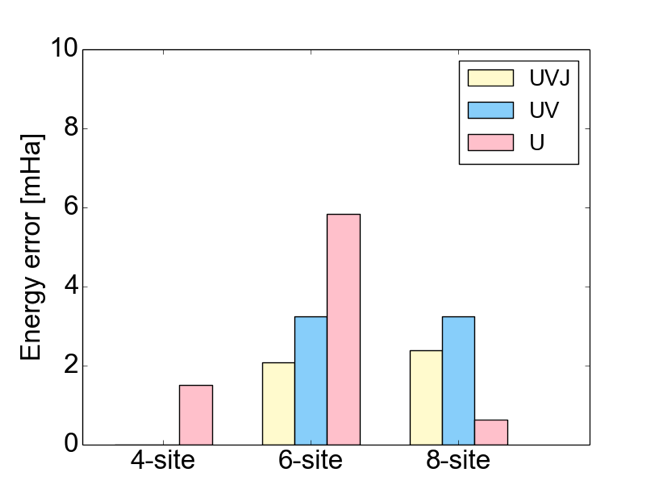
\includegraphics[width=0.40\linewidth]{h4_transfer_energy.png}}
%\caption{Errors of RDMs and energy for hydrogen chains with different number of sites: (a) relative error of two-body reduced density matrix; (b) error of eigen energy for $S=0$ and $S=1$ states per atom. the parameters used in model calculations are from 4-site chain.}\label{fig:h4transfer}
%\end{figure}
%In order to verify the transferability of the parameters for larger systems. We study longer chains (6-site, 8-site and 10-site) with the same inter-atomic distance (2\AA), and examine whether our parameters obtained from the 4-sites hydrogen chain is able to match the low energy physics of longer chains. We therefore, solve the model Hamiltonian with the parameters
%from Table.~\ref{tab:effm_hchain}, and examine the errors of the RDMs of S=0 and S=1 states. The results are
%shown in Fig.~\ref{fig:h4transfer}. As we can see, the error of the RDMs is around 10\%, indicating that the downfolding parameters from a smaller system is transferable to larger systems.
%Therefore, at $d=2$\AA, the hydrogen chain can be described by the extended Hubbard model \eqref{eq:h4model} very well. 

%As an alternative to the model-fitting approach for hydrogen given above, 
%we consider fitting a model to a periodic chain of 10 hydrogen atoms, but instead using low-energy states that do not explicitly target eigenstates of the Hamiltonian. In this example, 

We obtain single-particle Kohn-Sham orbitals from a set of spin-unrestricted and spin-restricted DFT-PBE calculations. With this set of orbitals, we produce a set of wave function states (\HHZ{Slater-Jastrow wave functions?}) consisting of singles- and doubles- excitations to the Slater determinant, %Allow $|KS \rangle $ to be the Slater determinant formed from the Kohn-Sham orbitals, and orbitals $i$ and $j$ ($k$ and $l$) to be Kohn-Sham orbitals that are unoccupied (occupied) in the Slater determinant. We then produce new wave function states as singles excitations $|s \rangle$ and doubles excitations $| d \rangle$ excitations to the Slater determinant:
\begin{subequations}
\begin{eqnarray}
| s \rangle = & \Big[a^\dagger_{i \sigma} a_{k \sigma}   | KS \rangle \Big]e^J \\
| d \rangle = & \: \Big[a^\dagger_{i \sigma} a^\dagger_{j \sigma'} a_{k \sigma'} c_{l \sigma}   | KS \rangle\Big]e^J ,
\end{eqnarray}
\end{subequations}
where $|KS\rangle$ is the Stater determinant of occupied Kohn-Sham orbitals, $\sigma$ and $\sigma'$ are spin indices and $a^\dagger$ ($a$) is a single-electron creation (destruction) operator corresponding to Kohn-Sham orbitals, and $e^J$ is the Jastrow factor which was optimized using variational Monte Carlo. This technique does not access the explicit eigenstates of the Hamiltonian, but allows many more states to be sampled in the process of characterizing the low-energy Hilbert of space of the system. The localized orbital basis upon which the descriptors are calculated is obtained by generating intrinsic atomic orbitals (IAO) from the Kohn-Sham orbitals, and localizing them using the L\"owdin localization procedure. \HHZ{Could you plot these orbitals and replace the Wannier orbitals stuff?}


%Having produced a set of wave functions, we compute the total energies and descriptor values associated to each parameter that might appear in the model. The \textit{ab-initio} Hamiltonian is solved using diffusion Monte Carlo (DMC) with Slater-Jastrow trial wave functions. Fig.~\ref{fig:Histogram-of-Parameter-Values} shows distributions for the $U$ and $t$ descriptors computed using this set of singly- and doubly-excited wave function states.  Because these descriptors vary in value between the distinct states we have constructed, it is appropriate to include both within a single model.
%
%\HHZ{We suggest to remove the discussion of covariance. Instead we could just show the results of Hubbard model fitting} There will exist some correlation between any two given descriptors. If two descriptors strongly covary with one another, then including both of them in a single model will introduce strong co-linearities, and produce aphysical parameter estimates. To control for this, we compute the covariance between descriptors prior to fitting a model, to verify that the descriptors are describing independent features of the wave function set. Fig.~\ref{fig:Cov-of-Descriptors} shows the absolute covariance of the hopping-$t$ descriptor with the $U$, $J$, and $V$ descriptors as a function of the separation distance between the hydrogen ions. We see that the covariance between the $t$ and $U$ descriptors is consistently low across all separation distances, indicating that these parameters are describing different wave function features. Therefore these descriptors are not strongly correlated with one another, and it is appropriate to include both in a single model.
%
Having computed the energies and descriptors for this set of wave functions, and verified the independence of the $U$ and $t$ descriptors, we fit a Hubbard-type model to describe the \textit{ab-initio} energetic results. Fig.~\ref{fig:RMS-Error-vs-Bond} shows the RMS error in the resultant $U$-$t$ model, relative to the \textit{ab-initio} DMC energetics, as a function of the hydrogen inter-atomic separation. We observe the the error is consistently less than 2 eV. The fitted value of the one-body hopping $t$ as a function of separation is shown in Fig.~\ref{fig:Parameters-vs-Bond-t}. As expected, the value of $t$ declines toward zero at larger separations. Hence, we see that the hydrogen chain can be well-described by a Hubbard-type model for a range of inter-atomic separations.

%\begin{figure}
%\centering
%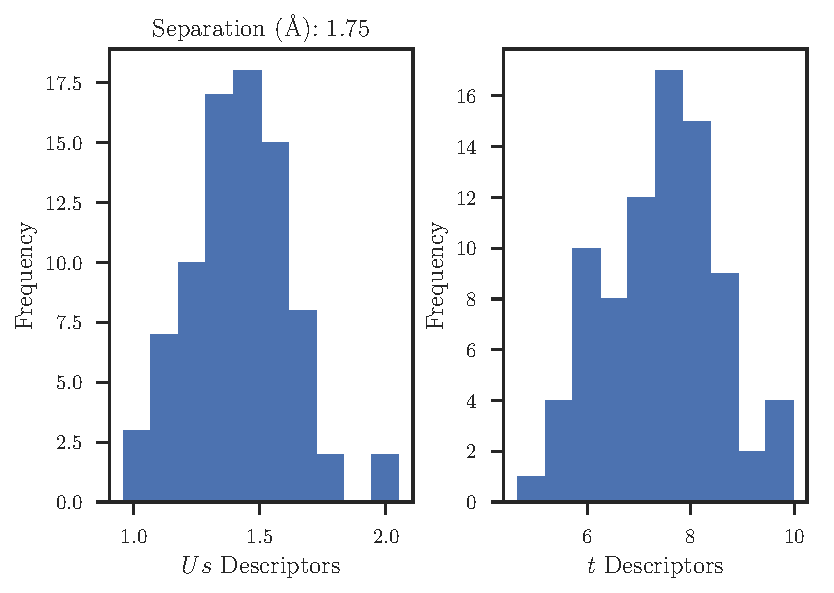
\includegraphics[scale=0.7]{./Figures/Spin0_pbe_H_relation.pdf}
%\caption{Histograms giving descriptor distributions for the one-body hopping $t$ and two-body Hubbard $U$ repulsion parameter for the periodic H$_{10}$ chain, with a lattice constant of $1.75$\AA.}\label{fig:Histogram-of-Parameter-Values}
% \end{figure}
% 
% \begin{figure}
%\centering
%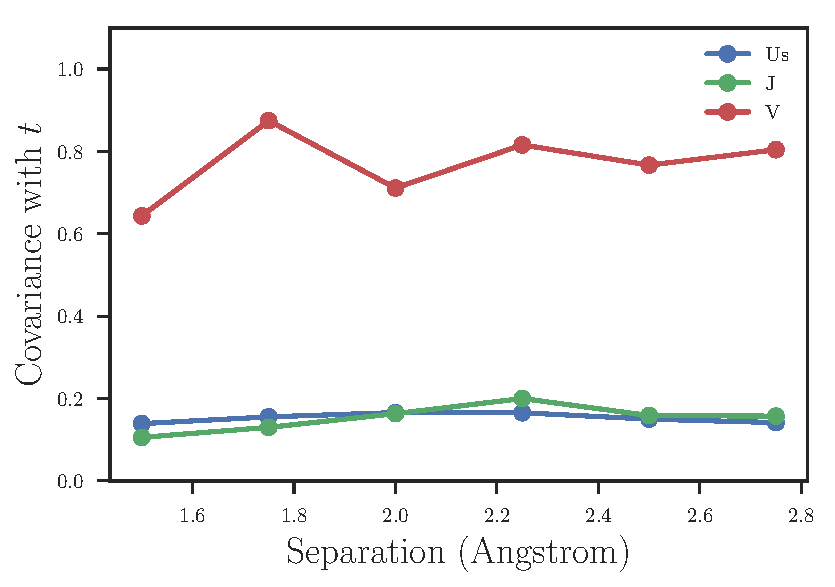
\includegraphics[scale=0.6]{./Figures/t_covariance_vs_separation.pdf}
%\caption{Covariance of the one-body hopping $t$ descriptor with the two-body $U$, $J$, and $V$ descriptors respectively, as a function of lattice constant for the periodic H$_{10}$ chain.  The covariance between the $t$ and $U$ is consistently small across all bond lengths.}\label{fig:Cov-of-Descriptors}
% \end{figure}
 
 \begin{figure}
\centering
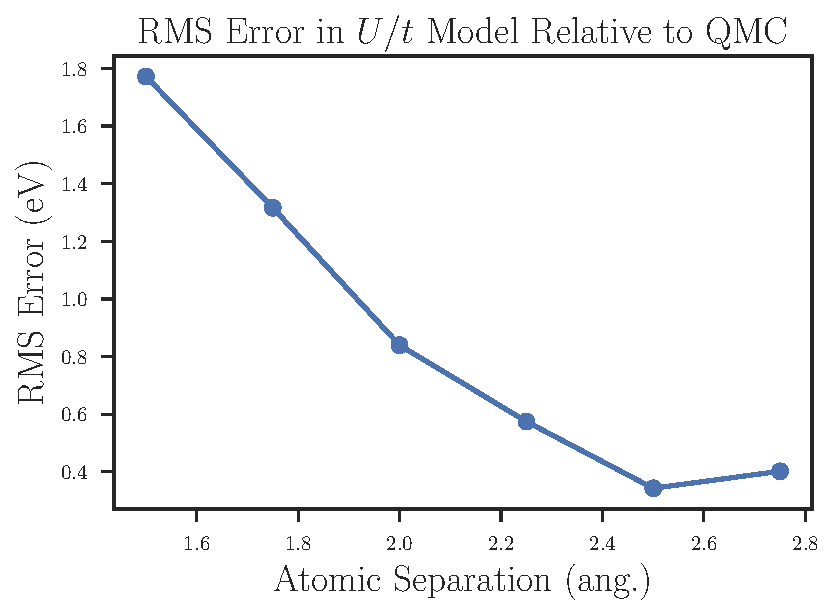
\includegraphics[scale=0.6]{./Figures/rms_ut_error_vs_separation_h_chain.pdf}
\caption{The RMS error in the fitted $U$-$t$ model for the periodic H$_{10}$ chain, relative to the \textit{ab-initio} energies. The RMS error is less than 1 eV for sufficiently long bond lengths.}\label{fig:RMS-Error-vs-Bond}
 \end{figure}
 
 \begin{figure}
\centering
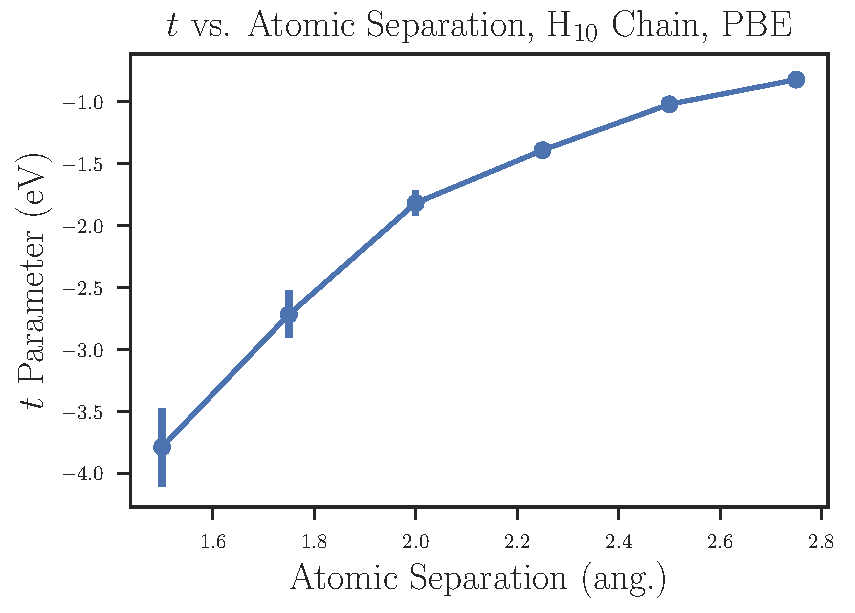
\includegraphics[scale=0.6]{./Figures/$t$_vs_separation_h_chain_ols.pdf}
\caption{The one-body hopping $t$ parameter as a function of lattice constant for the periodic H$_{10}$ chain, obtained from a fitted $U$-$t$ model. The parameter value declines to zero as the lattice constant increases. \HHZ{I suggest to remove the titles from the figure, and put description in the caption instead. The y-axis label: how about "Hopping parameter $t$"}}\label{fig:Parameters-vs-Bond-t}
 \end{figure}
